\documentclass[]{article}
\usepackage{lmodern}
\usepackage{amssymb,amsmath}
\usepackage{ifxetex,ifluatex}
\usepackage{fixltx2e} % provides \textsubscript
\ifnum 0\ifxetex 1\fi\ifluatex 1\fi=0 % if pdftex
  \usepackage[T1]{fontenc}
  \usepackage[utf8]{inputenc}
\else % if luatex or xelatex
  \ifxetex
    \usepackage{mathspec}
  \else
    \usepackage{fontspec}
  \fi
  \defaultfontfeatures{Ligatures=TeX,Scale=MatchLowercase}
\fi
% use upquote if available, for straight quotes in verbatim environments
\IfFileExists{upquote.sty}{\usepackage{upquote}}{}
% use microtype if available
\IfFileExists{microtype.sty}{%
\usepackage[]{microtype}
\UseMicrotypeSet[protrusion]{basicmath} % disable protrusion for tt fonts
}{}
\PassOptionsToPackage{hyphens}{url} % url is loaded by hyperref
\usepackage[unicode=true]{hyperref}
\hypersetup{
            pdfborder={0 0 0},
            breaklinks=true}
\urlstyle{same}  % don't use monospace font for urls
\usepackage{color}
\usepackage{fancyvrb}
\newcommand{\VerbBar}{|}
\newcommand{\VERB}{\Verb[commandchars=\\\{\}]}
\DefineVerbatimEnvironment{Highlighting}{Verbatim}{commandchars=\\\{\}}
% Add ',fontsize=\small' for more characters per line
\newenvironment{Shaded}{}{}
\newcommand{\KeywordTok}[1]{\textcolor[rgb]{0.00,0.44,0.13}{\textbf{#1}}}
\newcommand{\DataTypeTok}[1]{\textcolor[rgb]{0.56,0.13,0.00}{#1}}
\newcommand{\DecValTok}[1]{\textcolor[rgb]{0.25,0.63,0.44}{#1}}
\newcommand{\BaseNTok}[1]{\textcolor[rgb]{0.25,0.63,0.44}{#1}}
\newcommand{\FloatTok}[1]{\textcolor[rgb]{0.25,0.63,0.44}{#1}}
\newcommand{\ConstantTok}[1]{\textcolor[rgb]{0.53,0.00,0.00}{#1}}
\newcommand{\CharTok}[1]{\textcolor[rgb]{0.25,0.44,0.63}{#1}}
\newcommand{\SpecialCharTok}[1]{\textcolor[rgb]{0.25,0.44,0.63}{#1}}
\newcommand{\StringTok}[1]{\textcolor[rgb]{0.25,0.44,0.63}{#1}}
\newcommand{\VerbatimStringTok}[1]{\textcolor[rgb]{0.25,0.44,0.63}{#1}}
\newcommand{\SpecialStringTok}[1]{\textcolor[rgb]{0.73,0.40,0.53}{#1}}
\newcommand{\ImportTok}[1]{#1}
\newcommand{\CommentTok}[1]{\textcolor[rgb]{0.38,0.63,0.69}{\textit{#1}}}
\newcommand{\DocumentationTok}[1]{\textcolor[rgb]{0.73,0.13,0.13}{\textit{#1}}}
\newcommand{\AnnotationTok}[1]{\textcolor[rgb]{0.38,0.63,0.69}{\textbf{\textit{#1}}}}
\newcommand{\CommentVarTok}[1]{\textcolor[rgb]{0.38,0.63,0.69}{\textbf{\textit{#1}}}}
\newcommand{\OtherTok}[1]{\textcolor[rgb]{0.00,0.44,0.13}{#1}}
\newcommand{\FunctionTok}[1]{\textcolor[rgb]{0.02,0.16,0.49}{#1}}
\newcommand{\VariableTok}[1]{\textcolor[rgb]{0.10,0.09,0.49}{#1}}
\newcommand{\ControlFlowTok}[1]{\textcolor[rgb]{0.00,0.44,0.13}{\textbf{#1}}}
\newcommand{\OperatorTok}[1]{\textcolor[rgb]{0.40,0.40,0.40}{#1}}
\newcommand{\BuiltInTok}[1]{#1}
\newcommand{\ExtensionTok}[1]{#1}
\newcommand{\PreprocessorTok}[1]{\textcolor[rgb]{0.74,0.48,0.00}{#1}}
\newcommand{\AttributeTok}[1]{\textcolor[rgb]{0.49,0.56,0.16}{#1}}
\newcommand{\RegionMarkerTok}[1]{#1}
\newcommand{\InformationTok}[1]{\textcolor[rgb]{0.38,0.63,0.69}{\textbf{\textit{#1}}}}
\newcommand{\WarningTok}[1]{\textcolor[rgb]{0.38,0.63,0.69}{\textbf{\textit{#1}}}}
\newcommand{\AlertTok}[1]{\textcolor[rgb]{1.00,0.00,0.00}{\textbf{#1}}}
\newcommand{\ErrorTok}[1]{\textcolor[rgb]{1.00,0.00,0.00}{\textbf{#1}}}
\newcommand{\NormalTok}[1]{#1}
\usepackage{graphicx,grffile}
\makeatletter
\def\maxwidth{\ifdim\Gin@nat@width>\linewidth\linewidth\else\Gin@nat@width\fi}
\def\maxheight{\ifdim\Gin@nat@height>\textheight\textheight\else\Gin@nat@height\fi}
\makeatother
% Scale images if necessary, so that they will not overflow the page
% margins by default, and it is still possible to overwrite the defaults
% using explicit options in \includegraphics[width, height, ...]{}
\setkeys{Gin}{width=\maxwidth,height=\maxheight,keepaspectratio}
\IfFileExists{parskip.sty}{%
\usepackage{parskip}
}{% else
\setlength{\parindent}{0pt}
\setlength{\parskip}{6pt plus 2pt minus 1pt}
}
\setlength{\emergencystretch}{3em}  % prevent overfull lines
\providecommand{\tightlist}{%
  \setlength{\itemsep}{0pt}\setlength{\parskip}{0pt}}
\setcounter{secnumdepth}{0}
% Redefines (sub)paragraphs to behave more like sections
\ifx\paragraph\undefined\else
\let\oldparagraph\paragraph
\renewcommand{\paragraph}[1]{\oldparagraph{#1}\mbox{}}
\fi
\ifx\subparagraph\undefined\else
\let\oldsubparagraph\subparagraph
\renewcommand{\subparagraph}[1]{\oldsubparagraph{#1}\mbox{}}
\fi

% set default figure placement to htbp
\makeatletter
\def\fps@figure{htbp}
\makeatother


\date{}

\begin{document}

\section{基于Python语言的ARIMA模型算法}\label{header-c1}

\subsubsection{序}\label{header-c517}

时间序列数据在生产生活中极为常见。本文试图利用Python丰富的程序包,来建立适当的数学模型,对其进行描述和处理。

\subsubsection{1、时间序列模型与ARIMA模型}\label{header-c477}

时间序列的建模与预测在学术界和实际应用领域极为广泛。如股市价格、经济增长、人口数量等问题。1970年,美国的GEP
Box和GM
Jenkins发表了《\href{http://xueshu.baidu.com/s?wd=paperuri\%3A\%28715e90892dfadd5708d83ebc3e2110e2\%29\&filter=sc_long_sign\&tn=SE_xueshusource_2kduw22v\&sc_vurl=http\%3A\%2F\%2Fwww.ams.org\%2Fmathscinet-getitem\%3Fmr\%3D272138\&ie=utf-8\&sc_us=5034082631192868346}{Time
Series Analysis: Forecasting and
Control}》。自那以来,逐渐形成了一整套时间序列的估计、建模和预测的理论方法。

时间序列序列数据的存在和应用十分普遍,但是其数据特点却不完全相同,如果根据数据的特点,来建立合适的模型,以反应其特点、相对准确的预测其发展趋势,是时间序列分析中的重要问题。时间序列数学建模的理论,主要是建立在随机过程的基础之上;而计算机算法的发展,则为其建模带来的极大的方便。

时间序列数据模型中,最为普遍和简单的一种,就是ARIMA模型。

\subparagraph{1)自回归模型 (AR, autoregression)}\label{header-c92}

随机过程\{\(Y_t\)\}如果满足:
\(Y_t=c+\phi_1 \cdot Y_{t-1}+\mu_t\),且\(\mu_t\)的统计性质满足白噪音,则称\{\(Y_t\)\}为一个\(AR(1)\)过程。如果滞后项的阶数为\(p\),则为\(AR(p\))过程。

\subparagraph{2)移动平均模型 (MA, moving average)}\label{header-c100}

随机过程\({Y_t}\)如果满足:\(Y_t = c+\theta \cdot \mu_{t-1} + \mu_t\),且\(\mu_t\)的统计性质满足白噪音,则称\{\(Y_t\)\}为一个\(MA(q)\)过程。如果滞后项的阶数为\(q\),则为\(MA(q)\)过程。

\subparagraph{3)ARMA与ARIMA模型}\label{header-c108}

随机过程\({Y_t}\)如果满足:\(Y_t = c+\phi \cdot Y_{t-1}+ \theta \cdot \mu_{t-1} + \mu_t\),且\(\mu_t\)的统计性质满足白噪音,则称\{\(Y_t\)\}为一个\(ARMA(1,1)\)过程。如果自回归项的滞后阶数为\(p\),移动平均项滞后阶数为\(q\),则为\(ARMA(p,q)\)模型。

如果其中包含单位根过程,且单位根的阶数为1,则为\(ARIMA(p,1,q)\)过程。

当\(ARIMA(p,1,q)\)模型建立之后,通常需要对模型进行检验,以判断模型的拟合程度和预测准确度。通常的检验包括:

\subsubsection{2、Python语言处理时间序列模型}\label{header-c166}

下面试着用Python语言来处理时间序列模型。

首先导入计算模块。pandas, numpy, scipy,
和statsmodels是常用的数理统计模块,matplotlib则是常用的数据可视化的模块,在这里导入用来观察数据的趋势。

\begin{Shaded}
\begin{Highlighting}[]
\ImportTok{from}\NormalTok{ __future__ }\ImportTok{import}\NormalTok{ print_function}
\ImportTok{import}\NormalTok{ pandas }\ImportTok{as}\NormalTok{ pd}
\ImportTok{import}\NormalTok{ numpy }\ImportTok{as}\NormalTok{ np}
\ImportTok{from}\NormalTok{ scipy }\ImportTok{import}\NormalTok{  stats}
\ImportTok{import}\NormalTok{ matplotlib.pyplot }\ImportTok{as}\NormalTok{ plt}
\ImportTok{import}\NormalTok{ statsmodels.api }\ImportTok{as}\NormalTok{ sm}
\ImportTok{from}\NormalTok{ statsmodels.graphics.api }\ImportTok{import}\NormalTok{ qqplot}
\end{Highlighting}
\end{Shaded}

然后,输入数据。这是一个包含90个观测值的时间序列数据。

\begin{Shaded}
\begin{Highlighting}[]
\CommentTok{#input the data}
\NormalTok{dta}\OperatorTok{=}\NormalTok{[}\DecValTok{10930}\NormalTok{,}\DecValTok{10318}\NormalTok{,}\DecValTok{10595}\NormalTok{,}\DecValTok{10972}\NormalTok{,}\DecValTok{7706}\NormalTok{,}\DecValTok{6756}\NormalTok{,}\DecValTok{9092}\NormalTok{,}\DecValTok{10551}\NormalTok{,}\DecValTok{9722}\NormalTok{,}\DecValTok{10913}\NormalTok{,}\DecValTok{11151}\NormalTok{,}\DecValTok{8186}\NormalTok{,}\DecValTok{6422}\NormalTok{,}\DecValTok{6337}\NormalTok{,}\DecValTok{11649}\NormalTok{,}\DecValTok{11652}\NormalTok{,}\DecValTok{10310}\NormalTok{,}\DecValTok{12043}\NormalTok{,}\DecValTok{7937}\NormalTok{,}\DecValTok{6476}\NormalTok{,}\DecValTok{9662}\NormalTok{,}\DecValTok{9570}\NormalTok{,}\DecValTok{9981}\NormalTok{,}\DecValTok{9331}\NormalTok{,}\DecValTok{9449}\NormalTok{,}\DecValTok{6773}\NormalTok{,}\DecValTok{6304}\NormalTok{,}\DecValTok{9355}\NormalTok{,}\DecValTok{10477}\NormalTok{,}\DecValTok{10148}\NormalTok{,}\DecValTok{10395}\NormalTok{,}\DecValTok{11261}\NormalTok{,}\DecValTok{8713}\NormalTok{,}\DecValTok{7299}\NormalTok{,}\DecValTok{10424}\NormalTok{,}\DecValTok{10795}\NormalTok{,}\DecValTok{11069}\NormalTok{,}\DecValTok{11602}\NormalTok{,}\DecValTok{11427}\NormalTok{,}\DecValTok{9095}\NormalTok{,}\DecValTok{707}\NormalTok{,}\DecValTok{10767}\NormalTok{, }\DecValTok{12136}\NormalTok{,}\DecValTok{12812}\NormalTok{,}\DecValTok{12006}\NormalTok{,}\DecValTok{12528}\NormalTok{,}\DecValTok{10329}\NormalTok{,}\DecValTok{7818}\NormalTok{,}\DecValTok{11719}\NormalTok{,}\DecValTok{11683}\NormalTok{,}\DecValTok{12603}\NormalTok{,}\DecValTok{11495}\NormalTok{,}\DecValTok{13670}\NormalTok{,}\DecValTok{11337}\NormalTok{,}\DecValTok{10232}\NormalTok{,}\DecValTok{13261}\NormalTok{,}\DecValTok{13230}\NormalTok{,}\DecValTok{15535}\NormalTok{,}\DecValTok{16837}\NormalTok{,}\DecValTok{19598}\NormalTok{,}\DecValTok{14823}\NormalTok{,}\DecValTok{11622}\NormalTok{,}\DecValTok{19391}\NormalTok{,}\DecValTok{18177}\NormalTok{,}\DecValTok{19994}\NormalTok{,}\DecValTok{14723}\NormalTok{,}\DecValTok{15694}\NormalTok{,}\DecValTok{13248}\NormalTok{, }\DecValTok{9543}\NormalTok{,}\DecValTok{12872}\NormalTok{,}\DecValTok{13101}\NormalTok{,}\DecValTok{15053}\NormalTok{,}\DecValTok{12619}\NormalTok{,}\DecValTok{13749}\NormalTok{,}\DecValTok{10228}\NormalTok{,}\DecValTok{9725}\NormalTok{,}\DecValTok{14729}\NormalTok{,}\DecValTok{12518}\NormalTok{,}\DecValTok{14564}\NormalTok{,}\DecValTok{15085}\NormalTok{,}\DecValTok{14722}\NormalTok{, }\DecValTok{11999}\NormalTok{,}\DecValTok{9390}\NormalTok{,}\DecValTok{13481}\NormalTok{,}\DecValTok{14795}\NormalTok{,}\DecValTok{15845}\NormalTok{,}\DecValTok{15271}\NormalTok{,}\DecValTok{14686}\NormalTok{,}\DecValTok{11054}\NormalTok{,}\DecValTok{10395}\NormalTok{]}
\end{Highlighting}
\end{Shaded}

然后,我们对数据进行初步的检查和处理。

\begin{Shaded}
\begin{Highlighting}[]
\CommentTok{## change data type}
\NormalTok{dta}\OperatorTok{=}\NormalTok{np.array(dta,dtype}\OperatorTok{=}\NormalTok{np.}\BuiltInTok{float}\NormalTok{)}
\NormalTok{dta}\OperatorTok{=}\NormalTok{pd.Series(dta)}
\NormalTok{dta.index }\OperatorTok{=}\NormalTok{ pd.Index(sm.tsa.datetools.dates_from_range(}\StringTok{'1911'}\NormalTok{,}\StringTok{'2000'}\NormalTok{))}
\NormalTok{dta.plot(figsize}\OperatorTok{=}\NormalTok{(}\DecValTok{12}\NormalTok{,}\DecValTok{8}\NormalTok{))}
\CommentTok{# general view of the data}
\NormalTok{dta.plot(figsize}\OperatorTok{=}\NormalTok{(}\DecValTok{12}\NormalTok{,}\DecValTok{8}\NormalTok{))}
\NormalTok{plt.show()}
\end{Highlighting}
\end{Shaded}

可以得到下图:

\begin{figure}
\centering
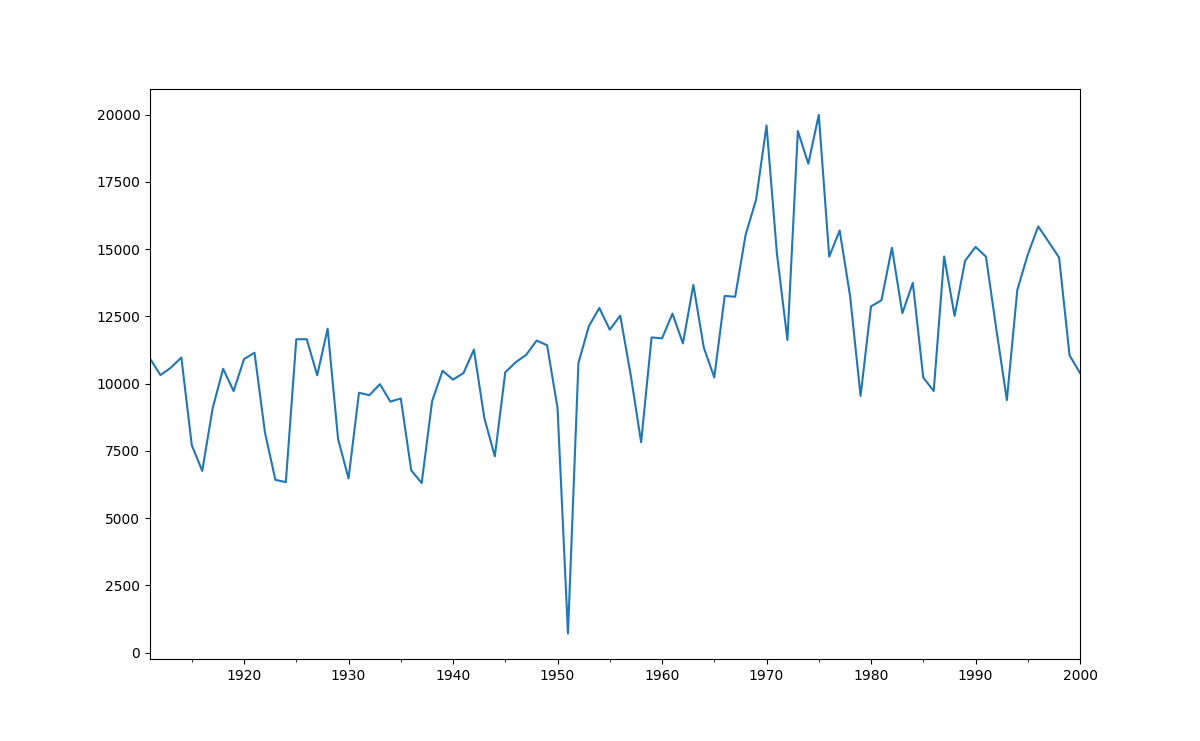
\includegraphics{F:/code/markdown/0312/figure_1.png}
\caption{}
\end{figure}

然后,我们对数据进行一阶差分,使其变得更为平稳。

\begin{Shaded}
\begin{Highlighting}[]
\CommentTok{## difference 1-order}
\NormalTok{fig }\OperatorTok{=}\NormalTok{ plt.figure(figsize}\OperatorTok{=}\NormalTok{(}\DecValTok{12}\NormalTok{,}\DecValTok{8}\NormalTok{))}
\NormalTok{ax1}\OperatorTok{=}\NormalTok{ fig.add_subplot(}\DecValTok{111}\NormalTok{)}
\NormalTok{diff1 }\OperatorTok{=}\NormalTok{ dta.diff(}\DecValTok{1}\NormalTok{)}
\NormalTok{diff1.plot(ax}\OperatorTok{=}\NormalTok{ax1)}
\NormalTok{plt.show()}
\end{Highlighting}
\end{Shaded}

\begin{figure}
\centering
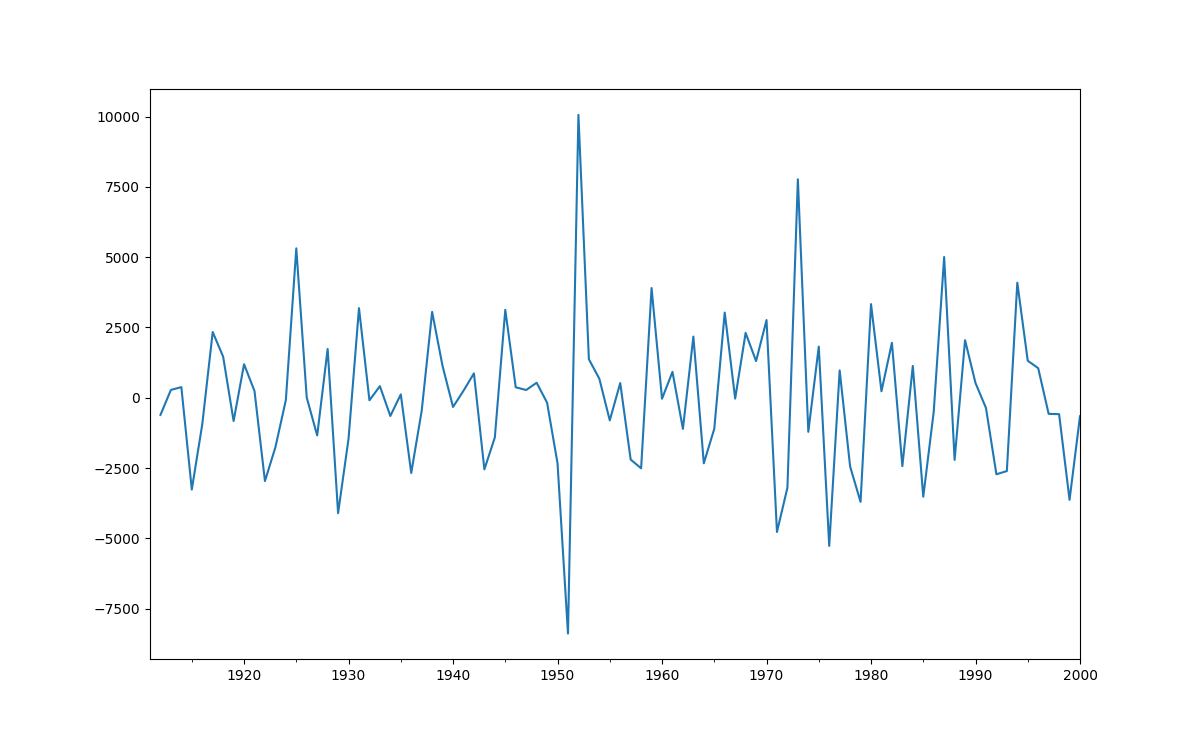
\includegraphics{F:/code/markdown/0312/figure_2.png}
\caption{}
\end{figure}

如果不满意,可以继续进行二阶差分。

\begin{Shaded}
\begin{Highlighting}[]
\CommentTok{## difference 2-order}
\NormalTok{fig }\OperatorTok{=}\NormalTok{ plt.figure(figsize}\OperatorTok{=}\NormalTok{(}\DecValTok{12}\NormalTok{,}\DecValTok{8}\NormalTok{))}
\NormalTok{ax2}\OperatorTok{=}\NormalTok{ fig.add_subplot(}\DecValTok{111}\NormalTok{)}
\NormalTok{diff2 }\OperatorTok{=}\NormalTok{ dta.diff(}\DecValTok{2}\NormalTok{)}
\NormalTok{diff2.plot(ax}\OperatorTok{=}\NormalTok{ax2)}
\NormalTok{plt.show()}
\end{Highlighting}
\end{Shaded}

\begin{figure}
\centering
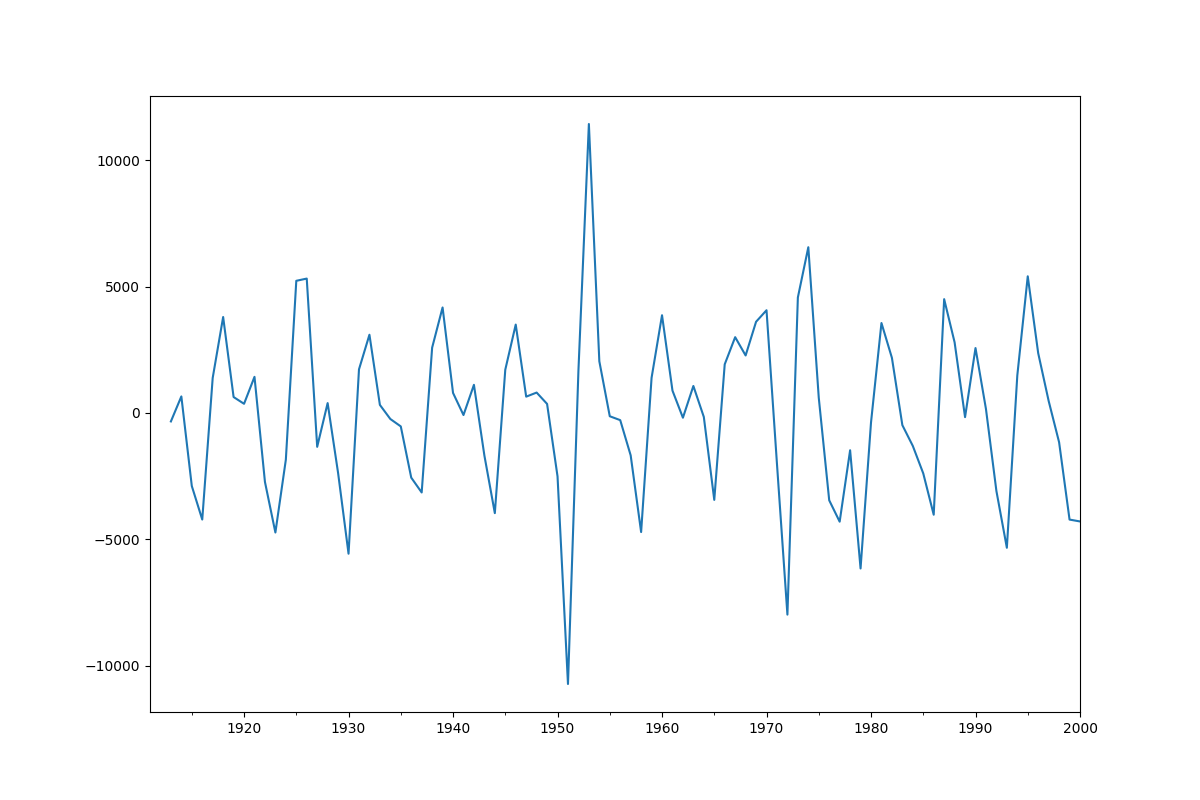
\includegraphics{F:/code/markdown/0312/figure_3.png}
\caption{}
\end{figure}

但是由于一阶差分的结果已经能够满足平稳,而且相对模型更为简单。所以之后的分析以一阶差分为基础。

为了确定自回归和移动平均的阶数,通常的一个简单的办法是观察自相关 (acf,
autocorrelation function) 和偏自相关(pacf, partial autocorrelation
funcition) 系数的情况。于是我们对一阶差分的acf和pacf作图观察。

\begin{Shaded}
\begin{Highlighting}[]
\CommentTok{## acf and pacf}
\NormalTok{diff1}\OperatorTok{=}\NormalTok{ dta.diff(}\DecValTok{1}\NormalTok{)}
\NormalTok{dta}\OperatorTok{=}\NormalTok{dta.diff1}
\NormalTok{fig }\OperatorTok{=}\NormalTok{ plt.figure(figsize}\OperatorTok{=}\NormalTok{(}\DecValTok{12}\NormalTok{,}\DecValTok{8}\NormalTok{))}
\NormalTok{ax1}\OperatorTok{=}\NormalTok{fig.add_subplot(}\DecValTok{211}\NormalTok{)}
\NormalTok{fig }\OperatorTok{=}\NormalTok{ sm.graphics.tsa.plot_acf(dta,lags}\OperatorTok{=}\DecValTok{40}\NormalTok{,ax}\OperatorTok{=}\NormalTok{ax1)}
\NormalTok{ax2 }\OperatorTok{=}\NormalTok{ fig.add_subplot(}\DecValTok{212}\NormalTok{)}
\NormalTok{fig }\OperatorTok{=}\NormalTok{ sm.graphics.tsa.plot_pacf(dta,lags}\OperatorTok{=}\DecValTok{40}\NormalTok{,ax}\OperatorTok{=}\NormalTok{ax2)}
\NormalTok{plt.show()}
\end{Highlighting}
\end{Shaded}

\begin{figure}
\centering
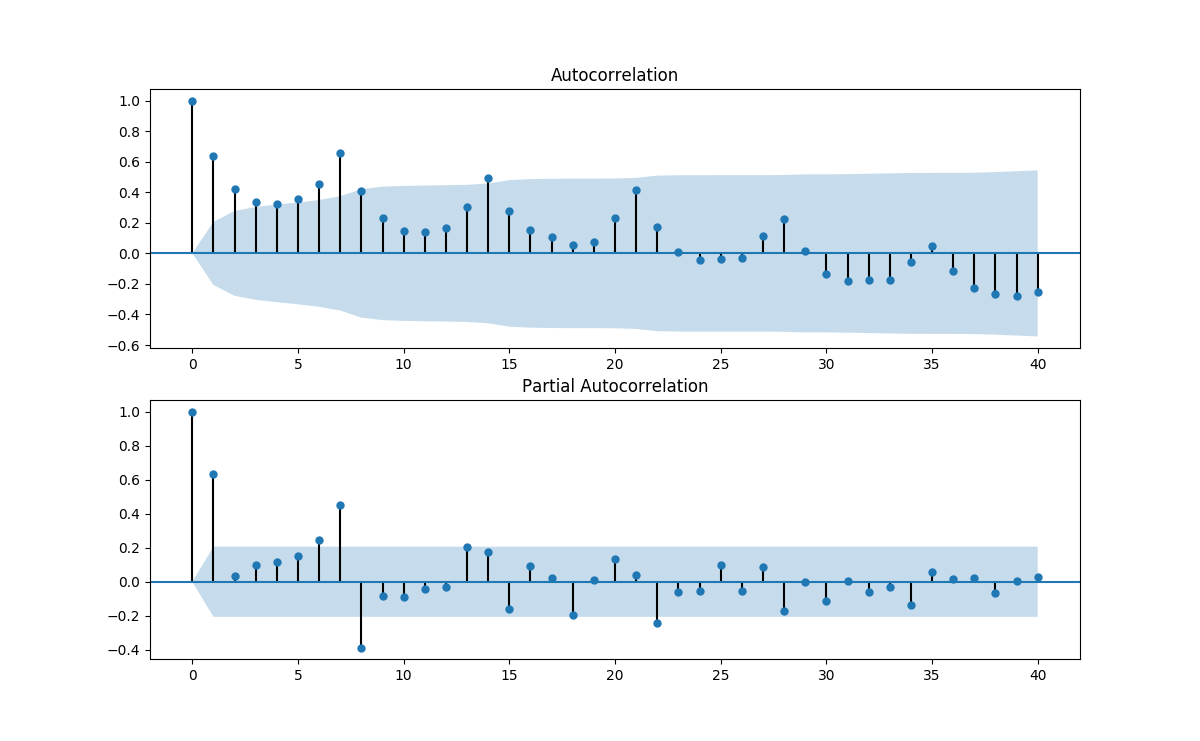
\includegraphics{F:/code/markdown/0312/figure_4.png}
\caption{}
\end{figure}

这里的自相关系数拖尾,偏自相关系数截尾,而且偏自相关在\(lag=8\)时有明显截尾的趋势,所以通过AIC和BIC准则对模型的\(AR(7)\)或\(AR(8)\)进行比较。

\begin{Shaded}
\begin{Highlighting}[]
\CommentTok{## model specification, AIC and BIC}
\NormalTok{arma_mod70 }\OperatorTok{=}\NormalTok{ sm.tsa.ARMA(dta,(}\DecValTok{7}\NormalTok{,}\DecValTok{0}\NormalTok{)).fit()}
\BuiltInTok{print}\NormalTok{(arma_mod70.aic,arma_mod70.bic,arma_mod70.hqic)}
\NormalTok{arma_mod30 }\OperatorTok{=}\NormalTok{ sm.tsa.ARMA(dta,(}\DecValTok{0}\NormalTok{,}\DecValTok{1}\NormalTok{)).fit()}
\BuiltInTok{print}\NormalTok{(arma_mod30.aic,arma_mod30.bic,arma_mod30.hqic)}
\NormalTok{arma_mod71 }\OperatorTok{=}\NormalTok{ sm.tsa.ARMA(dta,(}\DecValTok{7}\NormalTok{,}\DecValTok{1}\NormalTok{)).fit()}
\BuiltInTok{print}\NormalTok{(arma_mod71.aic,arma_mod71.bic,arma_mod71.hqic)}
\NormalTok{arma_mod80 }\OperatorTok{=}\NormalTok{ sm.tsa.ARMA(dta,(}\DecValTok{8}\NormalTok{,}\DecValTok{0}\NormalTok{)).fit() }
\BuiltInTok{print}\NormalTok{(arma_mod80.aic,arma_mod80.bic,arma_mod80.hqic)}
\end{Highlighting}
\end{Shaded}

最终确定AR的滞后阶数为8,MA的滞后阶数为0,即模型为\(ARIMA(8,1,0)\)模型(进行了一次差分)。

然后对模型进行进一步的检验。

\begin{itemize}
\item
  对残差的检验:通过残差的ACF和PACF可以看出,残差基本满足白噪声的条件。 
\end{itemize}

\begin{Shaded}
\begin{Highlighting}[]
\CommentTok{## residual}
\NormalTok{resid }\OperatorTok{=}\NormalTok{ arma_mod80.resid}
\NormalTok{fig }\OperatorTok{=}\NormalTok{ plt.figure(figsize}\OperatorTok{=}\NormalTok{(}\DecValTok{12}\NormalTok{,}\DecValTok{8}\NormalTok{))}
\NormalTok{ax1 }\OperatorTok{=}\NormalTok{ fig.add_subplot(}\DecValTok{211}\NormalTok{)}
\NormalTok{fig }\OperatorTok{=}\NormalTok{ sm.graphics.tsa.plot_acf(resid.values.squeeze(), lags}\OperatorTok{=}\DecValTok{40}\NormalTok{, ax}\OperatorTok{=}\NormalTok{ax1)}
\NormalTok{ax2 }\OperatorTok{=}\NormalTok{ fig.add_subplot(}\DecValTok{212}\NormalTok{)}
\NormalTok{fig }\OperatorTok{=}\NormalTok{ sm.graphics.tsa.plot_pacf(resid, lags}\OperatorTok{=}\DecValTok{40}\NormalTok{, ax}\OperatorTok{=}\NormalTok{ax2)}
\NormalTok{plt.show()}
\end{Highlighting}
\end{Shaded}

\begin{figure}
\centering
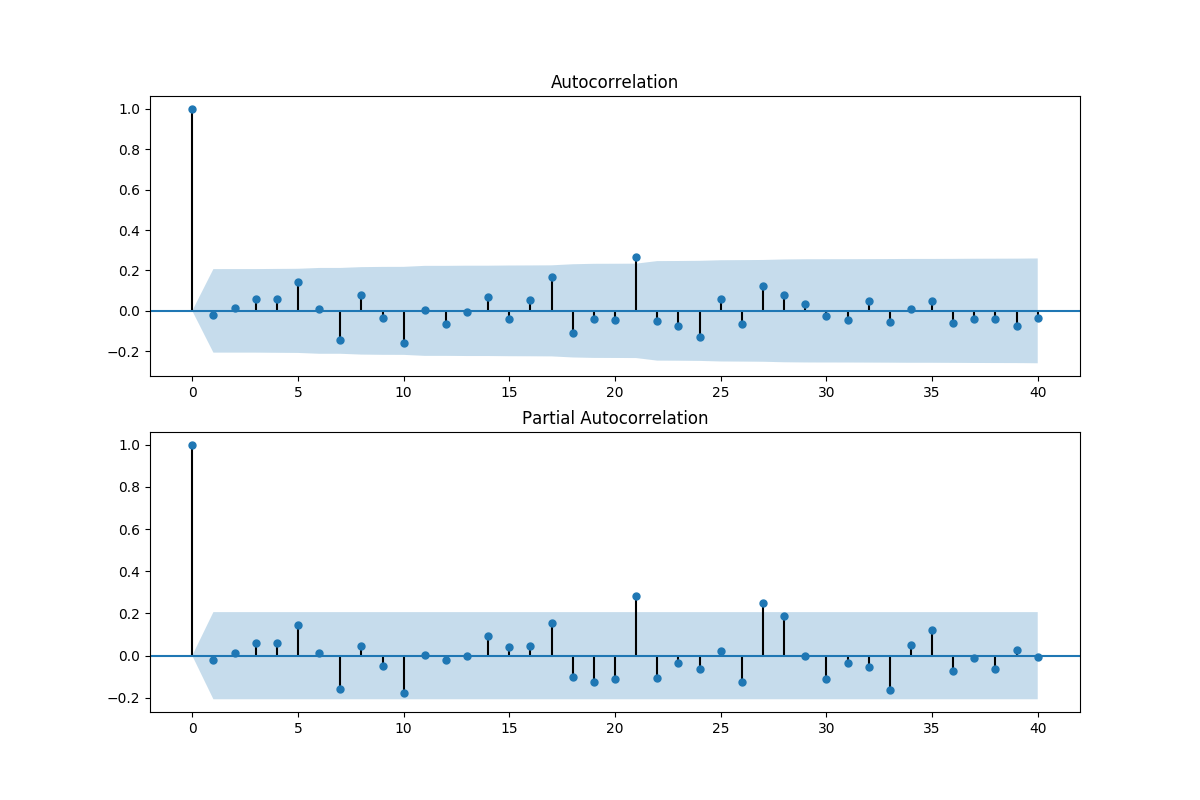
\includegraphics{F:/code/markdown/0312/figure_5.png}
\caption{}
\end{figure}

\begin{itemize}
\item
  对正态性的检验。结果看,正态性的条件符合得很好。

\begin{Shaded}
\begin{Highlighting}[]
\CommentTok{##Normarity test}
\BuiltInTok{print}\NormalTok{(stats.normaltest(resid))}
\NormalTok{fig }\OperatorTok{=}\NormalTok{ plt.figure(figsize}\OperatorTok{=}\NormalTok{(}\DecValTok{12}\NormalTok{,}\DecValTok{8}\NormalTok{))}
\NormalTok{ax }\OperatorTok{=}\NormalTok{ fig.add_subplot(}\DecValTok{111}\NormalTok{)}
\NormalTok{fig }\OperatorTok{=}\NormalTok{ qqplot(resid, line}\OperatorTok{=}\StringTok{'q'}\NormalTok{, ax}\OperatorTok{=}\NormalTok{ax, fit}\OperatorTok{=}\VariableTok{True}\NormalTok{)}
\NormalTok{plt.show()}
\end{Highlighting}
\end{Shaded}
\end{itemize}

\begin{quote}
NormaltestResult(statistic=14.604690828509506,
pvalue=0.00067395621352767988)
\end{quote}

\begin{figure}
\centering
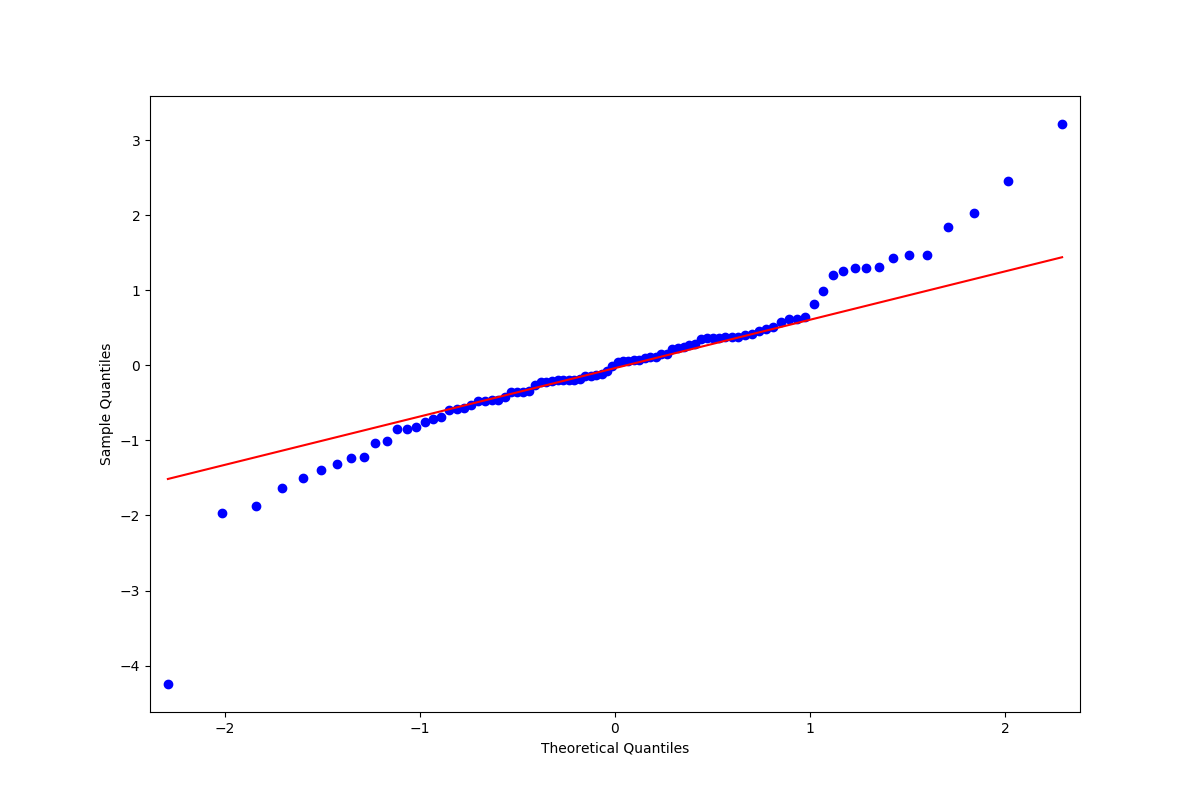
\includegraphics{F:/code/markdown/0312/figure_6.png}
\caption{}
\end{figure}

\begin{itemize}
\item
  D-W 检验。检验残差项的自相关情况。

\begin{Shaded}
\begin{Highlighting}[]
\CommentTok{##D-W test}
\BuiltInTok{print}\NormalTok{(sm.stats.durbin_watson(arma_mod80.resid.values))}
\end{Highlighting}
\end{Shaded}

  \begin{quote}
  2.04167903544
  \end{quote}
\item
  Ljunng-Box 检验。对模型的拟合效果进行综合检验。(输出略)

\begin{Shaded}
\begin{Highlighting}[]
\CommentTok{##Ljunng-Box test}
\NormalTok{r,q,p }\OperatorTok{=}\NormalTok{ sm.tsa.acf(resid.values.squeeze(), qstat}\OperatorTok{=}\VariableTok{True}\NormalTok{)}
\NormalTok{data }\OperatorTok{=}\NormalTok{ np.c_[}\BuiltInTok{range}\NormalTok{(}\DecValTok{1}\NormalTok{,}\DecValTok{41}\NormalTok{), r[}\DecValTok{1}\NormalTok{:], q, p]}
\NormalTok{table }\OperatorTok{=}\NormalTok{ pd.DataFrame(data, columns}\OperatorTok{=}\NormalTok{[}\StringTok{'lag'}\NormalTok{, }\StringTok{"AC"}\NormalTok{, }\StringTok{"Q"}\NormalTok{, }\StringTok{"Prob(>Q)"}\NormalTok{])}
\BuiltInTok{print}\NormalTok{(table.set_index(}\StringTok{'lag'}\NormalTok{))}
\end{Highlighting}
\end{Shaded}
\end{itemize}

\subsubsection{3、总结}\label{header-c13}

利用程序语言进行时间序列的分析,可以大大提高效率。在已有的成熟的统计软件如Stata/SAS/Eviews
等中,已经有了处理时间序列数据的相关内置函数或程序包,但是无论是计算效率、数据可视化的能力,还是灵活程度、开源性,都远远逊色于Python。本文仅仅对Python语言处理ARIMA模型进行简单的讨论和学习,希望能随着Python语言和算法的深入学习,掌握更多的处理ARIMA等时间序列模型的技巧。

\begin{center}\rule{0.5\linewidth}{\linethickness}\end{center}

\subsubsection{参考文献:}\label{header-c15}

\begin{enumerate}
\def\labelenumi{\arabic{enumi}.}
\item
  Autoregressive Moving Average (ARMA): Sunspots data, url:
  \url{http://statsmodels.sourceforge.net/devel/examples/notebooks/generated/tsa_arma_0.html\#autoregressive-moving-average-arma-sunspots-data.}
\item
  Python\_Statsmodels包\emph{时间序列分析}ARIMA模型,
  url:\url{http://blog.csdn.net/hal_sakai/article/details/51965657.}
\item
  {[}美{]}沃尔特·恩德斯(著),杜江、谢志超(译).应用计量经济学------时间序列分析(第2版),高等教育出版社.
\item
  涂云东,时间序列分析课堂讲义.
\item
  周广旭. (2005). 一种新的时间序列分析算法及其在股票预测中的应用.
  \emph{计算机应用}, \emph{25}(9), 2179-2181.
\end{enumerate}

\end{document}
